\documentclass[memey]{ali-presentation}

\usepackage{fontspec}
\usepackage{amsthm}
\usepackage{graphicx}

\hypersetup{
  colorlinks=true,
  allcolors=.,
  urlcolor=magenta,
}

\title{Overconfidence in Political Behavior}
\subtitle{Pietro Ortoleva and Erik Snowberg}

\date{March 11, 2026}
\author{Alistair Pattison}

\begin{document}

\maketitle

\section{Intro}

\begin{frame}
  \frametitle{This paper...}
  
  \begin{itemize}
    \item Studies the role of overconfidence in shaping ideology and political behavior.
    \item Develops a theoretical model linking overconfidence to:
      \begin{itemize}
        \item Ideological extremeness
        \item Higher voter turnout
        \item Stronger partisan identification
      \end{itemize}
    \item Generates and tests model predictions.
  \end{itemize}

\end{frame}

\begin{frame}
  \frametitle{Intuition}
  \begin{quote}
    ``For example, consider a
    citizen who notes the number of people in her neighborhood who are unemployed,
    and uses this information to deduce the state of the national economy. Suppose
    further that she lives in a neighborhood with high unemployment. If the citizen
    believes that the employment status of each person is relatively uncorrelated, she
    will think she has a lot of information about the state of the national economy
    (that is, she will be overconfident) and favor generous aid to the unemployed and
    loose monetary policy. If, instead, she realizes that local unemployment has a
    common cause—say, a factory shutting down—then she will understand that she
    has comparatively little information about the national economic situation, and
    believe that although the situation is bad, it is not likely to be dire, and will support
    more moderate policies.''
  \end{quote}
\end{frame}

\section{Data}

\begin{frame}
  \frametitle{Overconfidence Measure}

  \begin{itemize}
    \item Ask respondents questions with correct answers (e.g. current unemp. rate).
    \item Record accuracy and self-reported confidence in each answer.
    \item Define overconfidence as:
    $$
      \text{overconfidence} := \text{confidence} - \mathbb{E}[\text{confidence} \mid \text{accuracy}].
    $$
    \item Repeat for four questions in a survey with $n = 3{,}000$ respondents.
    \item Construct the first principal component to reduce measurement error.
  \end{itemize}
\end{frame}

\begin{frame}
  \frametitle{Overconfidence Measure}

  \begin{center}
    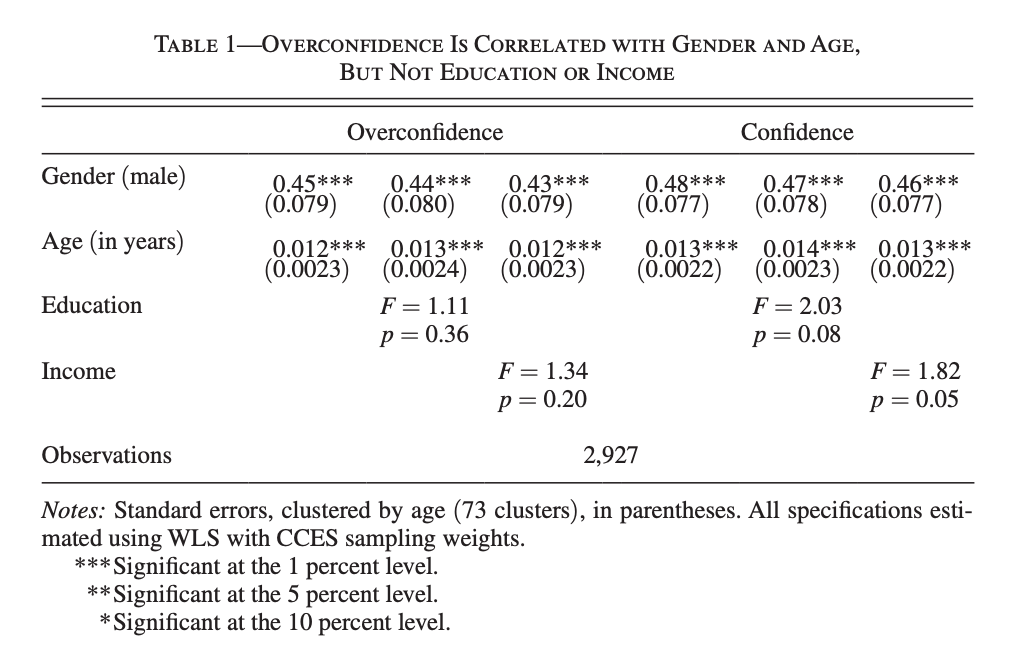
\includegraphics[height=2.5in]{figures/tbl-1.png}
  \end{center}
\end{frame}

\begin{frame}
  \frametitle{Other Data}

  \textit{Ideology}: (1) self-reported and (2) computed from 18 issue questions.

  \textit{Voter Turnout}: voting rolls.

  \textit{Partisan Identification}: self-report (strong/moderate/lean + Dem/Rep).

  \textit{Controls}: income, education, stock/home ownership, in union, state.

  \textit{Number of Signals}: media exposure, age.
\end{frame}

\section{Theoretical Framework}

\begin{frame}
  \frametitle{Basic Model}
  
  Each citizen $i$ has utility defined over actions $a_i$, some ``preference bias'' $b_i$, and some global state $x$:
  $$
    b_i \sim \mathcal N(0, \tau_b) \hspace{1in}
    x \sim \mathcal N(0, \tau)
  $$
  $$
    U(a_i, b_i \ | \ x) = - (a_i - b_i - x)^2.
  $$
  
  Define ideology to be the policy prefered by $i$
  $$
    \mathcal I_i = b_i + E_i[x]
  $$
  and extremeness
  $$
  \mathcal E_i = | \mathcal I_i |.
  $$

  % TODO: example?
\end{frame}

\begin{frame}
  \frametitle{Overconfidence}

  Everyone starts with the correct prior about $x \sim \mathcal N(0, \tau)$.
  Over time, people accumulate a vector of signals about $x$:
  $$
    (e_1, \ldots, e_n) \sim \mathcal N(x, \, \Sigma).
  $$
  People \emph{think} their experiences follow $\mathcal N(x, \, \Sigma')$ where $0 < \rho_i < \rho < 1$:

  $$
    \Sigma = \begin{pmatrix}
    1 & \rho & \cdots & \rho \\
    \rho & 1 & \cdots & \rho \\
    \vdots & \vdots & \ddots & \vdots \\
    \rho & \rho & \cdots & 1
    \end{pmatrix}
    \hspace{1in}
    \Sigma' = \begin{pmatrix}
    1 & \rho_i & \cdots & \rho_i \\
    \rho_i & 1 & \cdots & \rho_i \\
    \vdots & \vdots & \ddots & \vdots \\
    \rho_i & \rho_i & \cdots & 1
    \end{pmatrix}.
  $$
\end{frame}

\begin{frame}
  \frametitle{Similar to, but NOT Bayesian}

  In a Bayesian updating model, as $n \to \infty$, we should see
  \begin{itemize}
    \item overconfidence vanish
    \item all people converge to the same distribution (ideological spread vanish)
  \end{itemize}

  \pause

  In this model (Bayesian updating with incorrect liklihood), we should see
  \begin{itemize}
    \item overconfidence explode,
    \item spread explode (given sufficiently large experience correlation $\rho$)
  \end{itemize}
\end{frame}

\begin{frame}
  \frametitle{Intuition}

  Consider $\rho = 1$ and $\rho_i = 0$ (experiences are perfectly correlated, but people think they're independent). Then $n \to \infty$
  \begin{itemize}
    \item
      increases confidence without increasing information (so overconfidence increases),
    \item
      pushes people towards their biased perceptions (so spread increases).
  \end{itemize}
\end{frame}

\begin{frame}
  \frametitle{In the Data}

  \begin{center}
    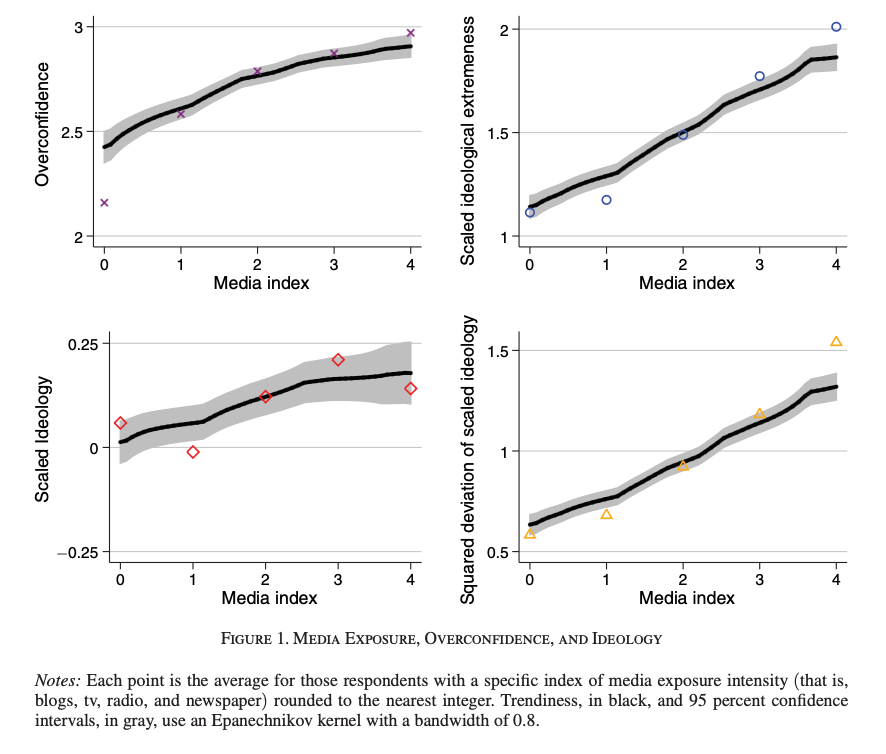
\includegraphics[width=3in]{figures/fig-1.png}
  \end{center}
\end{frame}

\section{Results}

\begin{frame}
  \frametitle{Overconfidence and Extremeness are Correlated}
  
  % TODO: fix this
  \begin{proposition}
    Overconfidence and ideological extremeness are positively correlated.
    This is true conditional on $n$, and independent of $n$ if $\rho$ is large enough
  \end{proposition}

  \begin{center}
    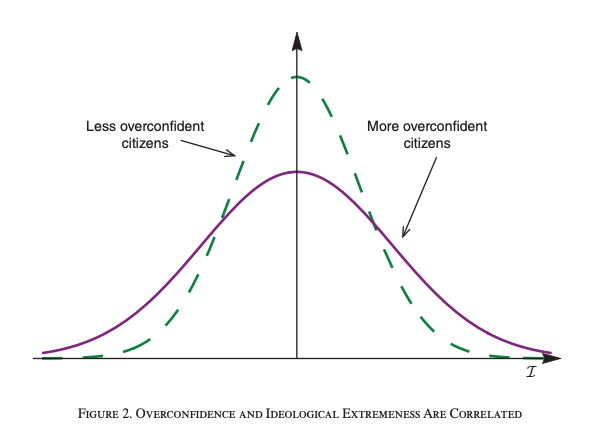
\includegraphics[height=2in]{figures/fig-2.png}
  \end{center}
\end{frame}

\begin{frame}
  \frametitle{In the Data}

  $$
    \text{Extremeness} := |\mathcal I_i - E[\mathcal I_i \ | \ \text{socioeconomic controls}]|
  $$

  \begin{center}
    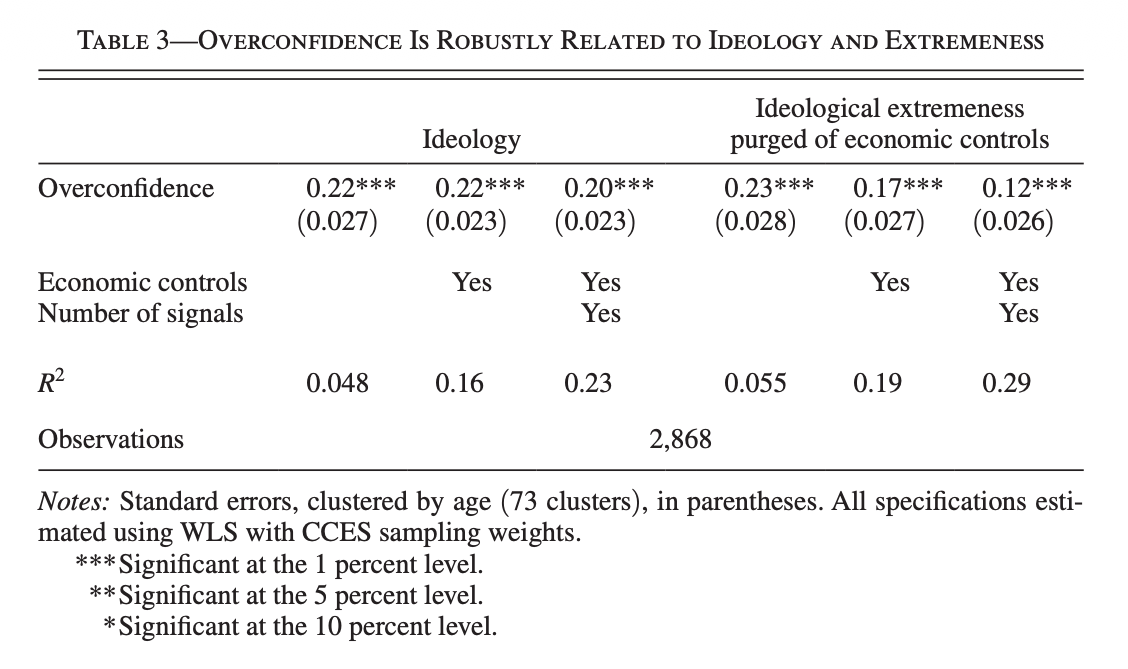
\includegraphics[height=2in]{figures/tbl-3.png}
  \end{center}
\end{frame}

\begin{frame}
  \frametitle{Effect Sizes in Context}
  
  \begin{center}
    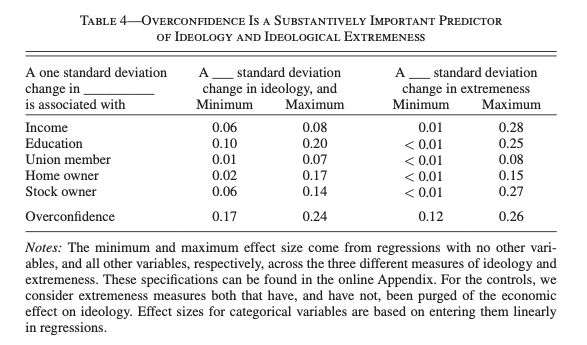
\includegraphics[height=2.5in]{figures/tbl-4.png}
  \end{center}
\end{frame}

\begin{frame}
  \frametitle{Voter Turnout}

  More overconfident citizens are more likely to turn out, even conditional on ideological extremeness.

  \begin{center}
    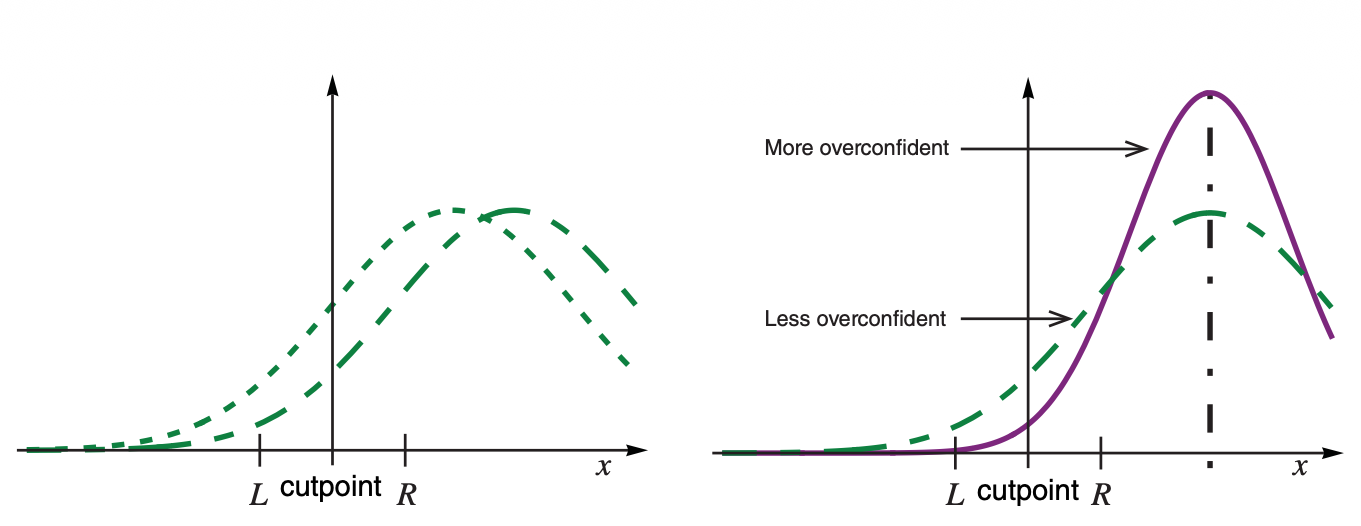
\includegraphics[width=5in]{figures/fig-4.png}
  \end{center}
\end{frame}

\begin{frame}
  \frametitle{Voter Turnout}

  \begin{center}
    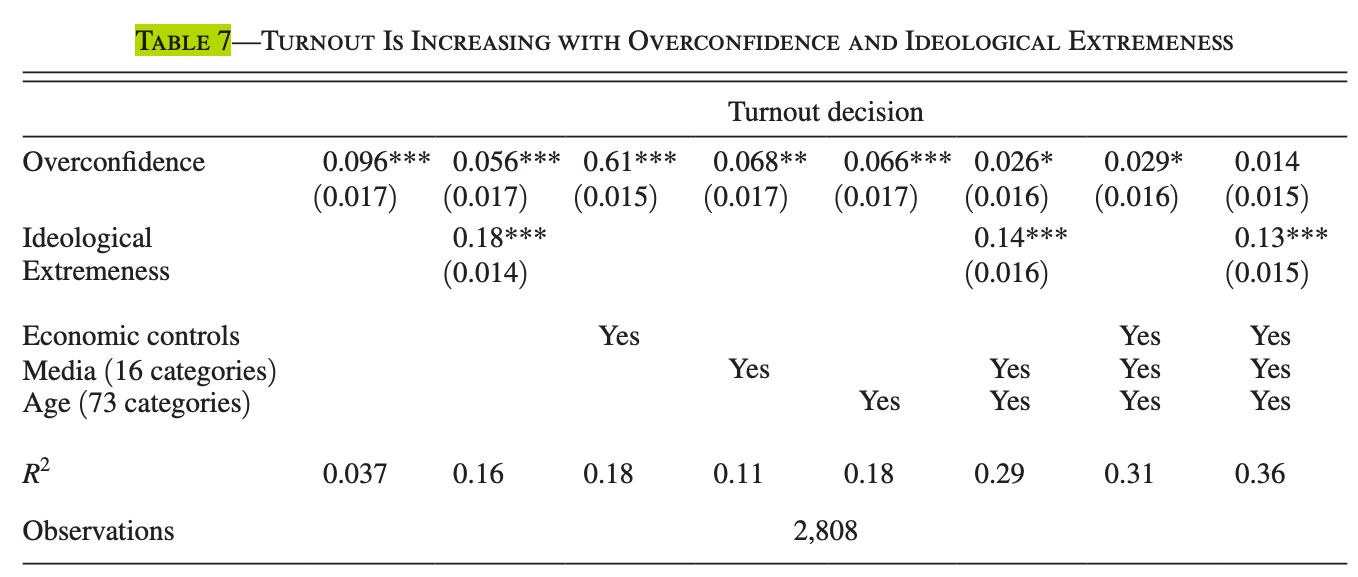
\includegraphics[width=5in]{figures/tbl-7.png}
  \end{center}
\end{frame}

\begin{frame}
  \frametitle{Other Things}

  \begin{itemize}
    \item Endoginizing media consumption ($n$) strengthens results.
    \item Sharing information
  \end{itemize}
\end{frame}

\end{document}
